\documentclass[11pt,a4paper]{report}
\usepackage[utf8]{inputenc}
\usepackage[T1]{fontenc}
\usepackage[english]{babel}
\usepackage[a4paper,margin=2.3cm]{geometry}
\usepackage{lmodern}
\usepackage{amsmath,amssymb}
\usepackage{graphicx,booktabs,float}
\IfFileExists{microtype.sty}{\usepackage{microtype}}{}
\IfFileExists{xurl.sty}{\usepackage{xurl}}{\usepackage{url}}
\usepackage[hidelinks]{hyperref}
\graphicspath{{output/report/}}
\setlength{\parindent}{0pt}
\setlength{\parskip}{0.6em}
\setlength{\emergencystretch}{2em}
\renewcommand{\arraystretch}{1.15}
\newcommand{\thetaT}{\theta}

\begin{document}
\hypersetup{pageanchor=false}
\begin{titlepage}
\centering
\vspace*{1.5cm}
{\Large \textsc{\'Ecole CentraleSup\'elec}\par}
\vspace{1.5cm}
{\Large Jules Andrevon--Canut and Ulysse Meyers\par}
\vspace{2cm}
\rule{\textwidth}{0.6pt}\par
\vspace{0.5cm}
{\huge\bfseries PIMC simulation of a proton in a one-dimensional double-well potential\par}
\vspace{0.5cm}
\rule{\textwidth}{0.6pt}\par
\vspace{1cm}
{\large Equilibrium distributions, effective barriers, and deterministic numerical checks\par}
\vfill
{\large 11 November 2026\par}
\end{titlepage}
\hypersetup{pageanchor=true}
\pagenumbering{roman}
\tableofcontents
\clearpage
\pagenumbering{arabic}

\chapter{Introduction}
Quantum tunneling and spatial delocalization influence the equilibrium behavior of light particles such as protons. In this project, a proton in a symmetric double-well potential is represented by a classical ring polymer and sampled with Path Integral Monte Carlo (PIMC). This equilibrium mapping incorporates quantum statistical effects through the imaginary-time path integral without simulating a real-time tunneling trajectory \cite{brief,ceperley}.

We study two values of the dimensionless quantum parameter, $C=0.3$ and $0.9$, and two reduced temperatures, $\theta=k_BT/V_0=0.4$ and $0.6$. The measured observables are the mean physical potential energy, the bead position density, and the centroid density. The centroid density defines an effective free-energy profile whose central barrier is compared with the bare barrier $V_0$.

The Monte Carlo results in this report were produced using a python notebook (\textit{main.ipynb}), and were compared with deterministic numerical references.

\chapter{Theoretical model and numerical method}
\section{Potential and physical scales}
The proton, of mass $m=m_p$, experiences
\begin{equation}
V(x)=V_0\left[\left(\frac{x}{a}\right)^2-1\right]^2,
\qquad a=0.04\,\mathrm{nm}.
\end{equation}
Its minima are at $x=\pm a$, and $V(0)=V_0$. Introduce $y=x/a$, $v(y)=V(x)/V_0=(y^2-1)^2$, and
\begin{equation}
C=\frac{\hbar^2}{2ma^2V_0},\qquad
\theta=\frac{k_BT}{V_0},\qquad
V_0=\frac{\hbar^2}{2ma^2C}.
\end{equation}
The code evaluates energies and positions in SI units. Reduced units are used here for interpretation, plotting, and deterministic references.
\begin{figure}[H]
\centering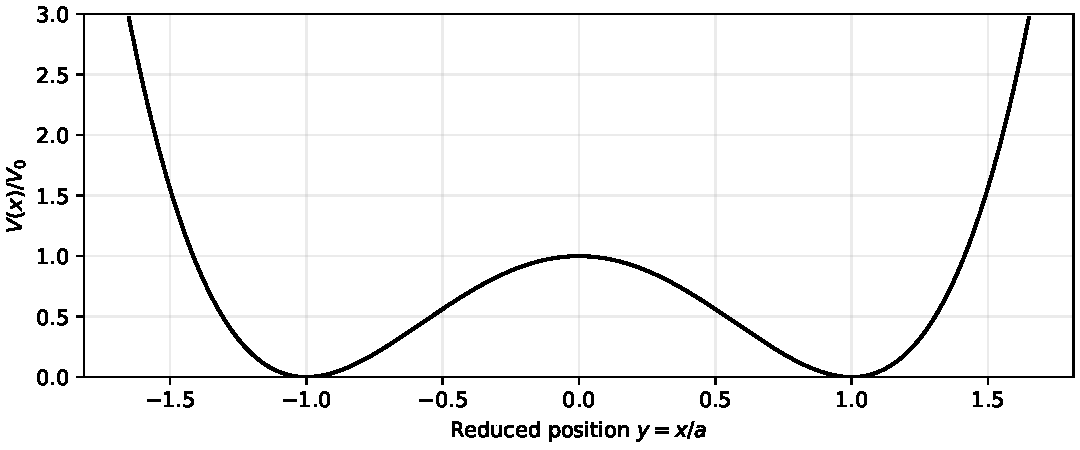
\includegraphics[width=0.83\linewidth]{double_well.pdf}
\caption{The reduced potential representing the double well.}
\label{fig:potential}
\end{figure}
Changing $C$ at fixed $m$ and $a$ changes $V_0$ and therefore the physical temperature corresponding to a fixed $\theta$:
\begin{center}
\begin{tabular}{rrrr}
\toprule
$C$ & $V_0$ (eV) & $T$ at $\theta=0.4$ (K) & $T$ at $\theta=0.6$ (K)\\
\midrule
0.3 & 0.043229 & 200.66 & 300.99\\
0.9 & 0.014410 & 66.89 & 100.33\\
\bottomrule
\end{tabular}
\end{center}
The two values of $C$ lie on opposite sides of the critical value $C_0\simeq0.732$ given in the project brief, where the ground-state total energy equals $V_0$ \cite{brief}. The deterministic spectrum below confirms this distinction.

\section{Ring-polymer action and Metropolis moves}
For $P$ beads, the effective energy sampled at inverse temperature $\beta=(k_BT)^{-1}$ is
\begin{equation}
U_{\mathrm{eff}}=\sum_{s=1}^P\left[
\frac12m\omega_P^2(x_{s+1}-x_s)^2+\frac{V(x_s)}{P}\right],
\quad \omega_P=\frac{\sqrt{P}k_BT}{\hbar},\quad x_{P+1}=x_1.
\end{equation}
This form can be found easily using the Trotter decomposition. \\
Equivalently,
\begin{equation}
\beta U_{\mathrm{eff}}=\sum_{s=1}^P\left[
\frac{P\theta}{4C}(y_{s+1}-y_s)^2+\frac{v(y_s)}{P\theta}\right].
\label{eq:action}
\end{equation}
A bead is selected uniformly at random and displaced by a uniform increment in $[-dx,dx]$. The move is accepted with probability $1$ if the new energy is lower, or with probability $e^{-\beta\Delta U_{\mathrm{eff}}}$ otherwise. Only the selected bead's potential and adjacent springs enter the energy difference. For $P=1$ the spring term vanishes. Initially all beads are at $x_s=a$.

One sweep comprises $P$ attempted moves with bead selection with replacement. Rejected moves remain part of the sampled trajectory. Histograms are recorded once per completed production sweep. Energy and centroid arrays are stored after every attempted move; an energy average after $B$ discarded sweeps therefore starts at array index $BP$. At $P=15$, 500,000 sweeps correspond to 7.5 million attempted moves.

\section{Observables and density convention}
The physical potential-energy estimator and centroid are
\begin{equation}
\langle V\rangle=\left\langle\frac1P\sum_sV(x_s)\right\rangle,
\qquad y_c=\frac1P\sum_s y_s.
\end{equation}
All beads contribute to the bead histogram; each configuration contributes one centroid. Both histograms use 100 bins over $y\in[-2.5,2.5]$ with width $\Delta y=0.05$. Their densities satisfy $\sum_i\rho_i\Delta y=1$ over this retained interval. The physical density is $\rho_x(x)=\rho_y(x/a)/a$. This common scale cancels in density ratios used for free energies.

The bead density approximates the quantum position density as $P$ increases. The centroid density describes the average position of an imaginary-time path, a distinct observable. Neither the $P$ beads within a configuration nor successive MC configurations should be assumed statistically independent.

\chapter{Classical validation and sampling protocol}
\section{Classical reference and displacement calibration}
At $P=1$, the target density and potential energy are
\begin{equation}
\rho_{\mathrm{cl}}(y)=\frac{e^{-v(y)/\theta}}{\int e^{-v(y)/\theta}\,dy},
\qquad \langle v\rangle_{\mathrm{cl}}=\int v(y)\rho_{\mathrm{cl}}(y)\,dy.
\end{equation}
Question 3 evaluates these integrals with the trapezoidal rule on 2,001 points in $[-2.5,2.5]$. At $\theta=0.4$ this gives $\langle V\rangle_{\mathrm{cl}}/V_0=0.228637092$. Refinement to 4,001 points on $[-3,3]$ leaves the displayed value unchanged.

The tested maximum displacements are $dx/a=0.2,0.4,0.8,1.0,1.2,1.6,2.0,2.4,3.0$. Each pilot uses 20,000 attempted moves, of which the first 5,000 are excluded from the acceptance and crossing diagnostics. The value closest to 45\% acceptance is $dx=a$, with measured acceptance 44.7\%. This is a practical calibration, rather than a proof of optimal sampling efficiency: larger proposed moves produce more well crossings in the pilot.
\begin{figure}[H]
\centering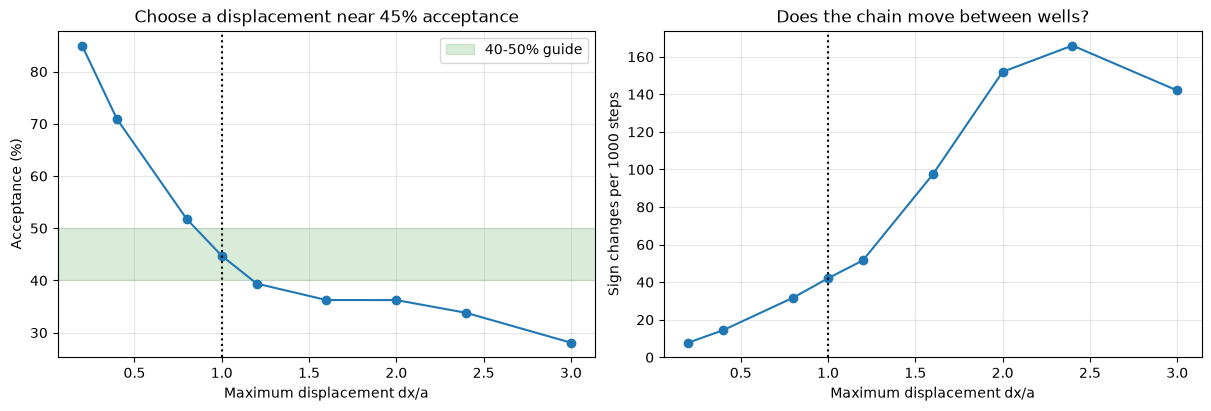
\includegraphics[width=\linewidth]{classical_tuning.png}
\caption{Displacement calibration.}
\end{figure}
Three subsequent classical runs use 200,000 attempted moves each and discard 5,000. Their saved summaries are:
\begin{center}
\begin{tabular}{rrrr}
\toprule
Seed & $\langle x\rangle/a$ & $\langle V\rangle/V_0$ & Fraction in right well\\
\midrule
10 & $-0.0110$ & 0.2292 & 0.494\\
20 & $-0.0004$ & 0.2268 & 0.500\\
30 & $-0.0256$ & 0.2276 & 0.486\\
\bottomrule
\end{tabular}
\end{center}
The means and histogram support agreement with the classical reference. The green bands in Figure~\ref{fig:classical} represent chosen accuracy goals ($|\langle x\rangle|<0.05a$ and energy within 5\% of the reference), not confidence intervals.
\begin{figure}[H]
\centering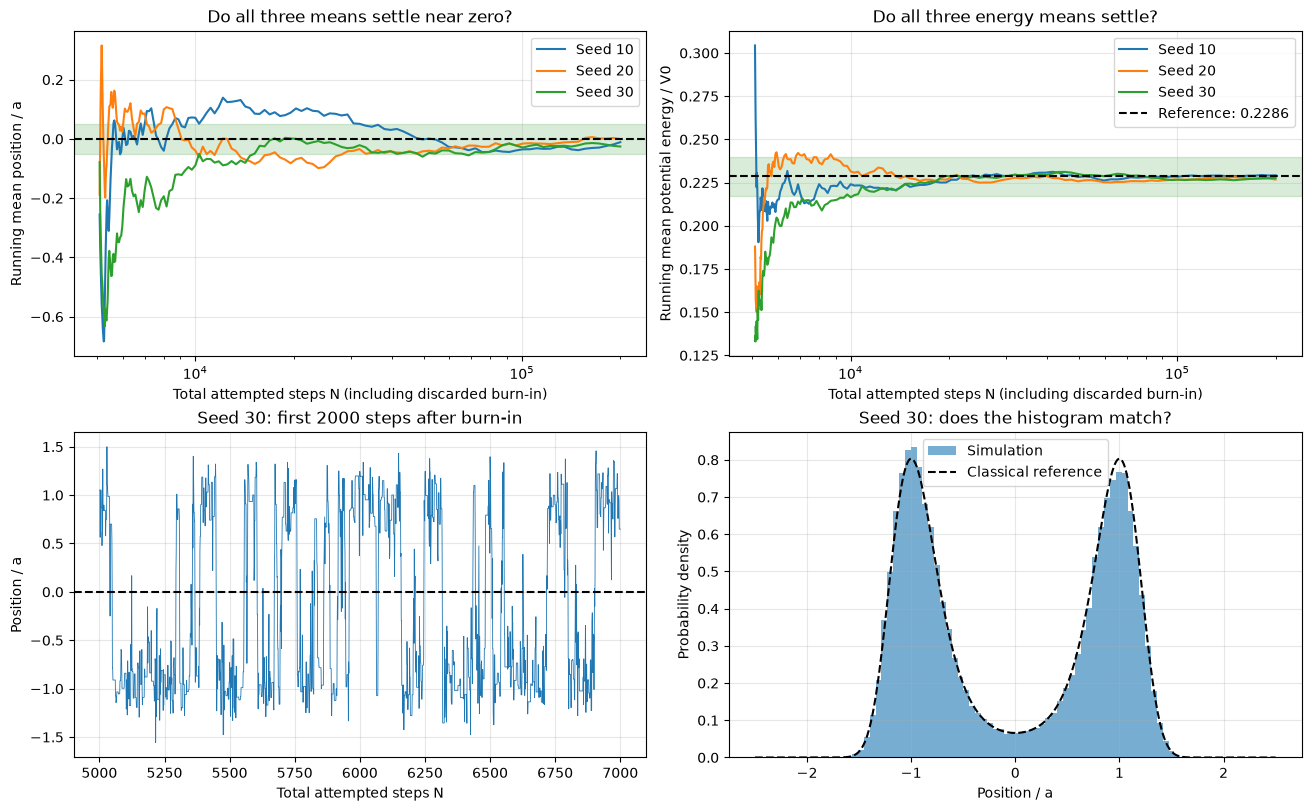
\includegraphics[width=\linewidth]{classical_validation.png}
\caption{Number of steps calibration. Plot 3.2.c shows the jump between the two wells.}
\label{fig:classical}
\end{figure}

\section{Protocols used for the quantum experiments}
The production displacement rule is
\begin{equation}
\frac{dx}{a}=0.4\sqrt{\frac{50}{P}}\,a_{\mathrm{corr}},\qquad a_{\mathrm{corr}}=1.
\end{equation}
where $0.4$ and $50$ were manually tuned to give approximately 45\% acceptance at $P=50$.\\
Thus $dx\simeq0.730a$ at $P=15$. Final acceptances are around 45\%.
\begin{table}[H]
\centering\small
\begin{tabular}{lrrl}
\toprule
Experiment & Discarded sweeps & Production sweeps & Repetitions\\
\midrule
$P$ scan, $C=0.3$, $\theta=0.4$ & 5,000 & 25,000 & 5 runs\\
$P$ scan, $C=0.9$, $\theta=0.4$ & 5,000 & 25,000 & 5 runs\\
Final distributions, $\theta=0.4$ & 100,000 & 400,000 & Seeds 10, 20, 30\\
Final distributions, $\theta=0.6$ & 100,000 & 400,000 & Seed 20\\
\bottomrule
\end{tabular}
\caption{Actual MC schedules.}
\label{tab:schedules}
\end{table}
An earlier 50,000-sweep distribution test at $C=0.3$, $\theta=0.4$ discarded 5,000 sweeps, which result in a strongly asymetric distribution. The sampling was not good enough, thus it was changed to 500,000 sweeps. The report uses the subsequent longer experiments. At the lower temperature three centroid densities are averaged before taking their logarithm. The standard deviation of the three individual barrier estimates is reported as run-to-run spread.

\chapter{Results and comparison}
\section{Convergence with bead count}
At $\theta=0.4$, saved MC scans cover $P=1$ to $32$ for $C=0.3$ and to $40$ for $C=0.9$. Both show an increasing mean potential energy followed by a noisy plateau. The five individual runs and their mean are plotted.
\begin{figure}[H]
\centering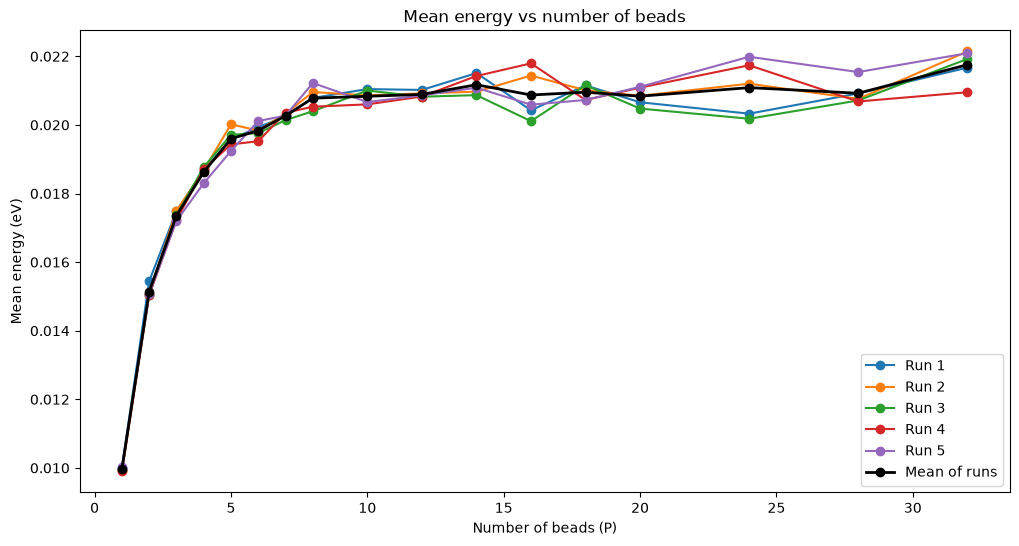
\includegraphics[width=0.91\linewidth]{mc_energy_C03.png}
\caption{Saved MC potential-energy scan at $C=0.3$, $\theta=0.4$. The vertical axis is in eV.}
\label{fig:mcscan}
\end{figure}
\begin{figure}[H]
\centering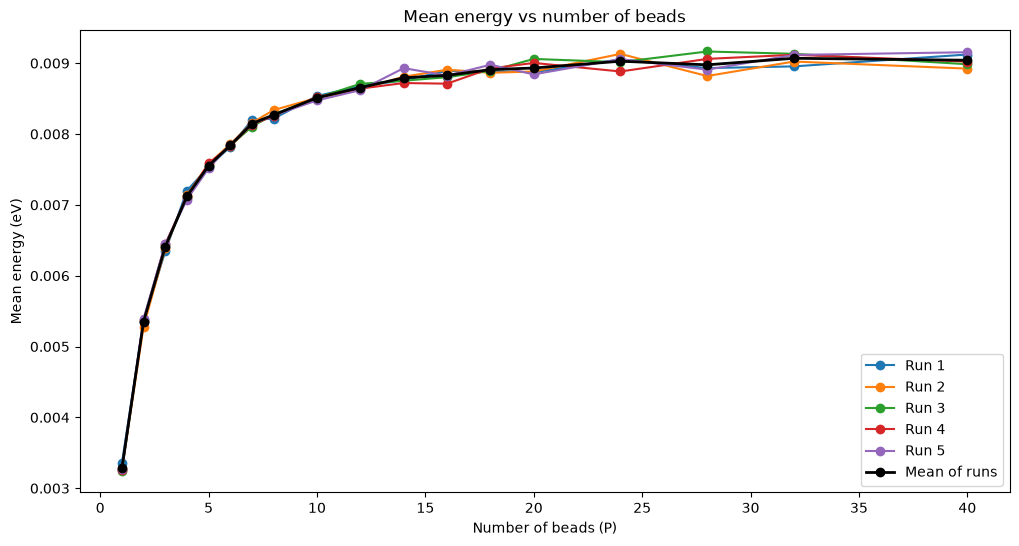
\includegraphics[width=0.91\linewidth]{mc_energy_C09.png}
\caption{Saved MC potential-energy scan at $C=0.9$, $\theta=0.4$.}
\end{figure}
All final MC distributions use $P=15$ as a practical compromise. The deterministic finite-$P$ reference gives potential-energy underestimates of about 1.23\% for $C=0.3$ and 3.40\% for $C=0.9$ at $\theta=0.4$. At $\theta=0.6$ the corresponding biases are about 0.57\% and 1.73\%. These discretization biases persist even with perfect MC sampling.
\begin{figure}[H]
\centering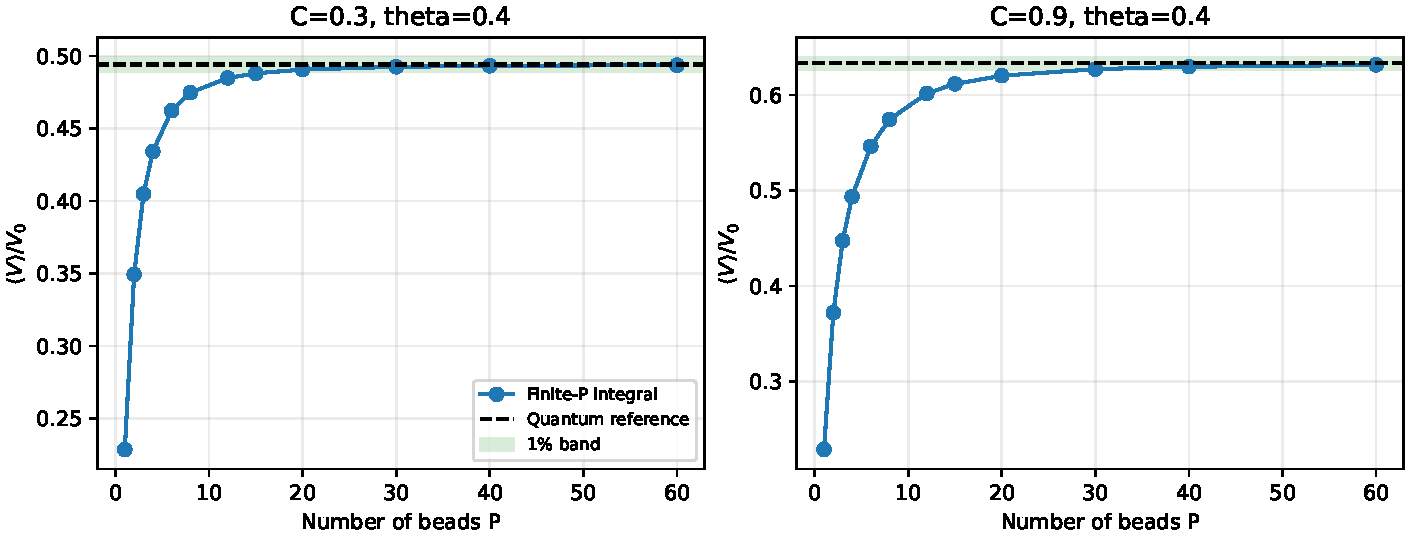
\includegraphics[width=\linewidth]{reference_energy_convergence.pdf}
\caption{Deterministic finite-$P$ potential energies, the Schr\"odinger reference, and a 1\% band. Unlike a noisy MC plateau, this comparison directly isolates the finite-$P$ effect.}
\end{figure}
The saved MC $P$ scans were not repeated at $\theta=0.6$, and the measured centroid densities were not compared across $P$.

\section{Bead and centroid distributions}
For $C=0.3$, $\theta=0.4$, the measured bead density has two broad peaks shifted inward from the classical potential minima and an increased probability near the central barrier. The centroid density has narrower outer tails and sharper peaks near the wells. These differences reflect fluctuations of the beads about their centroid.
\begin{figure}[H]
\centering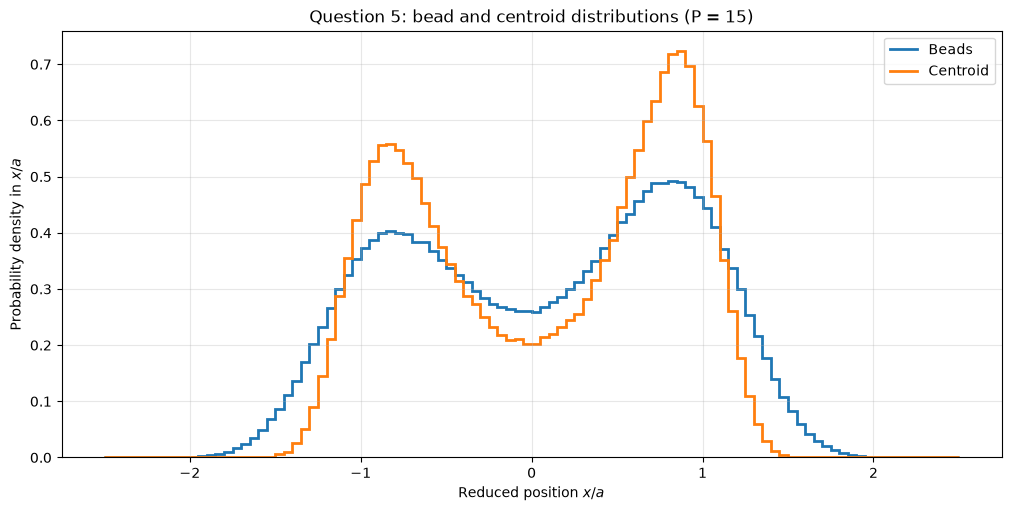
\includegraphics[width=0.95\linewidth]{mc_distribution_C03.png}
\caption{Saved $P=15$ distributions for $C=0.3$, $\theta=0.4$, seed 10, after 100,000 discarded and 400,000 production sweeps. This individual run is shown to expose the residual population imbalance.}
\label{fig:dist03}
\end{figure}
The unequal peak heights in Figure~\ref{fig:dist03} are not a physical breaking of the symmetry: $V(y)=V(-y)$ implies symmetric equilibrium densities. Their variation across seeds is evidence of sampling uncertainty, particularly for the relative populations of the two wells. A normalized histogram area of one does not resolve this problem.
\begin{figure}[H]
\centering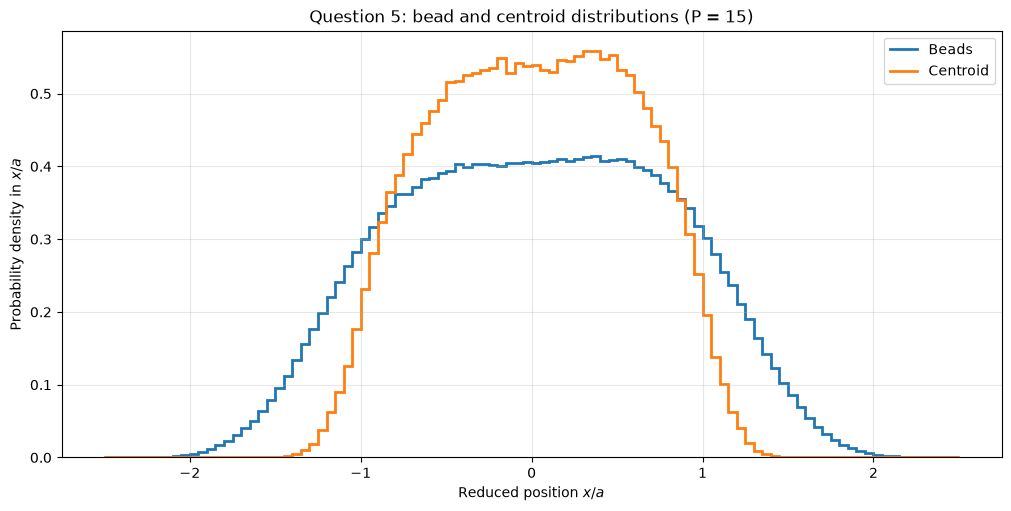
\includegraphics[width=0.95\linewidth]{mc_distribution_C09.png}
\caption{Saved $P=15$ distributions for $C=0.9$, $\theta=0.4$, seed 10, with the same sweep schedule.}
\label{fig:dist09}
\end{figure}
For $C=0.9$ the distribution is broader around the origin and the centroid barrier is strongly suppressed. The deterministic quantum-limit bead density has its maximum at the origin at $\theta=0.4$, while finite-$P$ effects and MC fluctuations can produce a shallow or nearly flat central structure. At $\theta=0.6$ the centroid density regains a shallow two-peak shape.

\section{Effective barriers and their uncertainties}
The centroid free-energy profile is defined up to a constant:
\begin{equation}
\frac{F_c(q)}{V_0}=-\theta\ln\!\left[\frac{\rho_c(q)}{\rho_{c,\max}}\right].
\end{equation}
For a symmetric bimodal density, the barrier is the difference between the central maximum of $F_c$ and its two equal minima. At $P=1$, the exact density gives $F_c(y)=V(y)$ and bare barrier $V_0$.

The implemented finite-bin estimator uses the bin $[0,0.05]$, centered at $0.025$, and the maximum histogram bin density. It approximates the central value, rather than evaluating exactly at zero. With a sampled asymmetric density it also refers to the deeper sampled minimum. Empty histogram bins are masked in the pooled lower-temperature profiles; the existing higher-temperature cells still emit logarithm warnings in empty tails. These tail bins do not enter the reported central estimates.
\begin{table}[H]
\centering\small
\begin{tabular}{rrrrrrr}
\toprule
$C$ & $\theta$ & Runs & MC & Run SD & Reference $P=15$ & Reference $P=60$\\
\midrule
0.3 & 0.4 & 3 & 0.458 & 0.050 & 0.425299 & 0.421468 \\
0.3 & 0.6 & 1 & 0.6184 & -- & 0.577325 & 0.575023 \\
0.9 & 0.4 & 3 & 0.012 & 0.006 & 0.000000 & 0.000000 \\
0.9 & 0.6 & 1 & 0.1395 & -- & 0.098754 & 0.093603 \\
\bottomrule
\end{tabular}
\caption{Central-bin barriers divided by $V_0$. Lower-temperature MC values use pooled densities; higher-temperature values use one seed. Run SD is the standard deviation of individual run estimates; a dash means it was not estimated. The deterministic references match the MC bins.}
\label{tab:barriers}
\end{table}

For $C=0.3$, the pooled lower-temperature barrier is $0.458V_0$, and the three individual estimates are $0.509V_0$, $0.410V_0$, and $0.461V_0$. Their standard deviation is $0.050V_0$, illustrating the remaining statistical variability. For $C=0.9$, the corresponding values are $0.014V_0$, $0.023V_0$, and $0.012V_0$, with pooled estimate $0.012V_0$ and standard deviation $0.006V_0$. These spreads must not be interpreted as confidence intervals for the pooled estimator.

The matched deterministic $P=15$ reference is lower than the saved MC barrier in every case. Thus the discrepancy cannot be explained solely by finite-$P$ bias: it is present even when comparing the same discretized path integral and bins. Slow centroid sampling, imbalanced well populations, and selection of the largest noisy density bin are plausible contributors. Quantifying their effects would require additional statistical analysis.
\begin{figure}[H]
\centering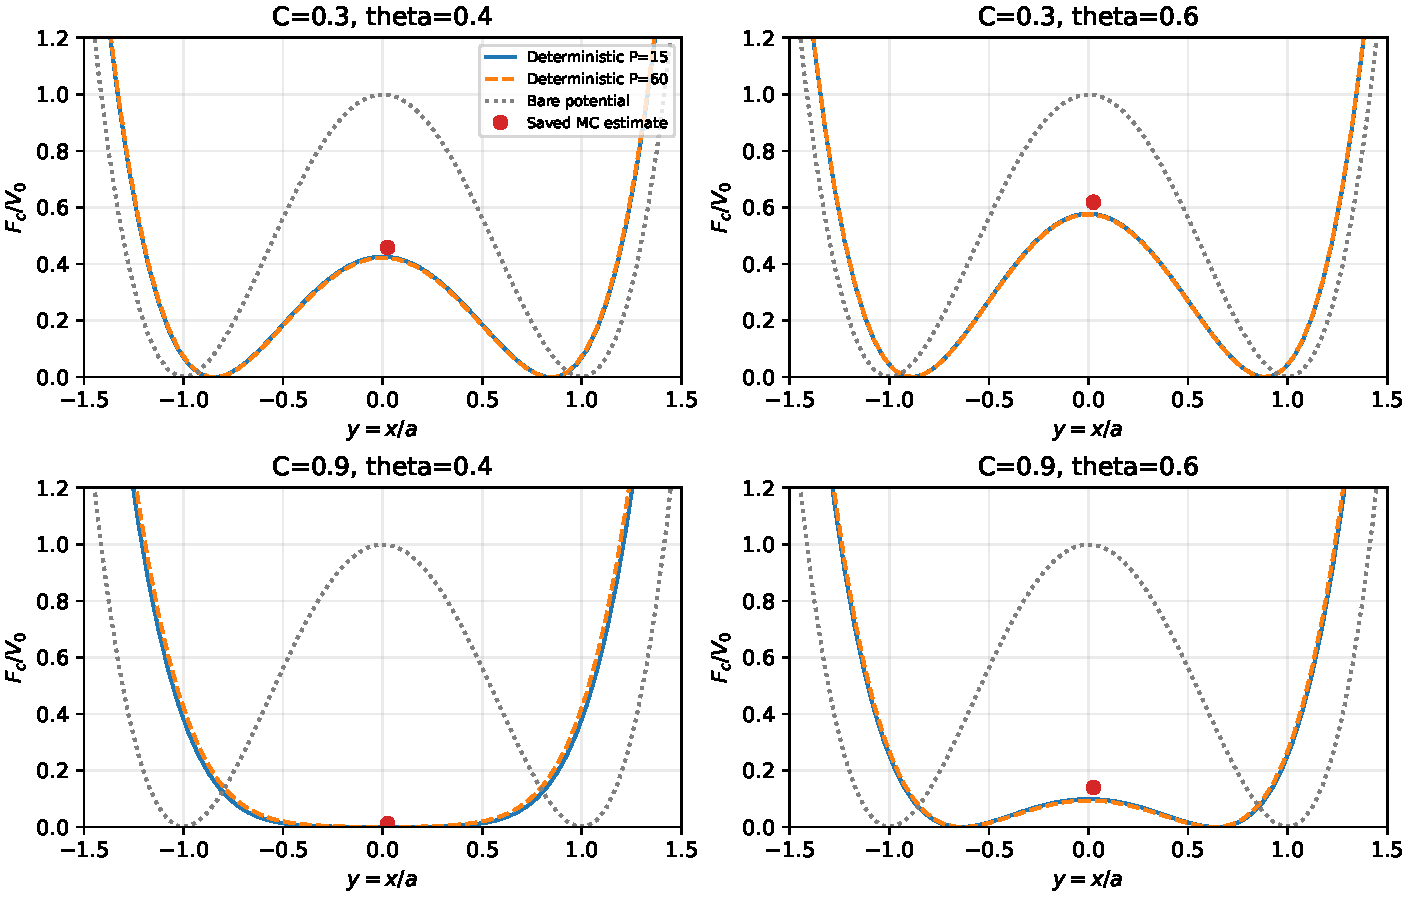
\includegraphics[width=\linewidth]{reference_barriers.pdf}
\caption{Deterministic centroid free energies at $P=15$ and $60$, the bare potential, and the saved MC central-bin estimates. MC markers show estimates without confidence intervals. The references use the same bins as the MC.}
\label{fig:barriers}
\end{figure}
The saved barriers increase with temperature for both values of $C$, while increasing $C$ at fixed reduced temperature reduces them. The deterministic references support these trends. At $C=0.9$, $\theta=0.4$, the reference centroid density peaks at the center, so there is no resolved central barrier; the small positive MC value is compatible with a nearly flat profile and sampling noise. At the higher temperature the shallow centroid barrier is restored. These comparisons concern reduced temperatures, whose physical values differ between the two choices of $C$.

\chapter{Discussion and conclusion}
The implemented Metropolis updates reproduce the classical distribution and potential-energy reference to the accuracy suggested by three independent runs. The quantum calculations show greater bead delocalization, distinct bead and centroid densities, and an effective barrier substantially below the bare value $V_0$.

The deterministic section added to the notebook makes the reference values reproducible and separates two errors. The finite-difference Schr\"odinger solution determines quantum-limit potential energies and bead densities. The transfer matrix integrates the same finite-$P$ path distribution as the MC and supplies a direct benchmark for its centroid estimator. These checks establish that $P=15$ has measurable discretization bias and that some remaining barrier discrepancies arise within the finite-$P$ sampling problem itself.

The evidence supports a decreasing centroid barrier with increasing $C$ and an increasing barrier with temperature in the cases studied. It does not establish uniform 1\% accuracy, an optimal bead count, or confidence intervals for the barriers. Residual asymmetry, a short discarded transient in one bead-count scan, unequal replication across temperatures, and the absence of autocorrelation or block analysis remain limitations. Collective path moves, replicated higher-temperature runs, and observable-specific convergence checks are appropriate next steps. PIMC determines equilibrium quantum statistics; its MC steps and centroid free-energy profiles do not directly give real-time tunneling rates.

\begin{thebibliography}{9}
\bibitem{brief} H. Dammak, \emph{Mod\'elisation et Simulation Num\'erique}, Chapter 8, ``PIMC applied to a simple 1D system. Double well potential. Tunnel effect (IK)'', project brief, pp.~21--22.
\bibitem{ceperley} D. M. Ceperley, ``Path integrals in the theory of condensed helium,'' \emph{Reviews of Modern Physics} \textbf{67}, 279--355 (1995). \url{https://doi.org/10.1103/RevModPhys.67.279}.
\bibitem{scipy} SciPy documentation, \texttt{scipy.linalg.eigh\_tridiagonal}, \url{https://docs.scipy.org/doc/scipy/reference/generated/scipy.linalg.eigh_tridiagonal.html}.
\end{thebibliography}
\end{document}
